\section{Digitale Regler}

Betrachtung \textbf{quasi-kontinuierlicher Regler}, d.h. \(T_A \le \frac{1}{10} \ldots \frac{1}{20} \cdot T_{System, dom}\) \\
(\(T_{System, dom}\) ist die dominierende (größte) Zeitkonstante des Systems)

\subsection{z-Transformation}

	Wert der bei t = k $\cdot T_A$ ausgegeben wird, wird bei t = (k-1) $\cdot T_A$
	eingelesen. (Verzögerung um einen Abtastschritt):

	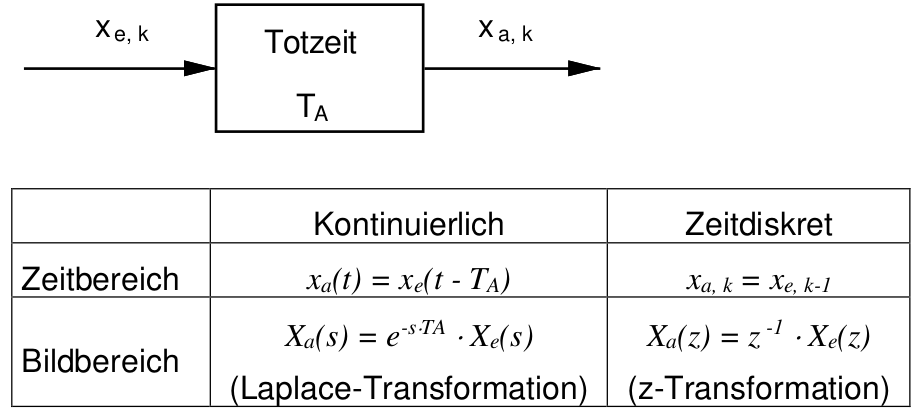
\includegraphics[width=0.9\columnwidth]{Figures/digitaleRegler/zTrans.png}

	\begin{align*}
		\Rightarrow &z \ \hat{=}\  e^{s \cdot T_A} \\
		\text{bzw. } &s \ \hat{=}\  \frac{1}{T_A} \cdot \ln(z)
	\end{align*}

	Um die Übertragungsfunktion eines digitalen Reglers zu erhalten, wird für \(s\) ein entsprechender Ausdruck in Abhängigkeit von \(z\) und der Abtastzeit \(T_A\) eingesetzt. \\ 
	Zur Vereinfachung der Berechnung von digitalen Reglern können folgende Näherungsformeln verwendet werden:

	\begin{itemize}
		\item Rückwärts-Differenzen-Quotient: \(s \ \hat{=} \ \frac{z-1}{T_A \cdot z}\)
		\item Vorwärts-Differenzen-Quotient: \(s \ \hat{=} \ \frac{z-1}{T_A}\)
		\item Tustinsche Formel: \(s \ \hat{=} \ \frac{2}{T_A} \cdot \frac{z-1}{z+1}\)
	\end{itemize}

	\subsubsection{Stabilität von digitalen Reglern}
		Ein digitaler Regler ist stabil, wenn alle Pole innerhalb des Einheitskreises liegen, d.h. \(|z| < 1\). \\
		\textbf{Beispiel:} \(G(z) = \frac{z}{z-0.5}\) hat einen Pol bei \(z = 0.5\) und ist damit stabil, da \(|0.5| < 1\). \\
		\textbf{Beispiel:} \(G(z) = \frac{z}{z-1.5}\) hat einen Pol bei \(z = 1.5\) und ist damit instabil, da \(|1.5| > 1\).

\subsection{Algorithmus aus der Übertragungsfunktion}
	\begin{itemize}
		\item Übertragungsfunktion in z-Form umwandeln
		\item Zähler und Nenner durch die höchste Potenz von z teilen (Es darf nur \(z^0, z^{-1}, z^{-2} \ldots\) geben, kein \(z^{+\ldots}\))
		\item Zähler gibt Eingangsgrößen an, Nenner gibt Ausgangsgrößen an, z.B. \(\frac{2+4z^{-1}}{8-5z^{-1}} \ \Rightarrow \ 8 x_{a,k} - 5 x_{a,k-1} = 2 x_{e,k} + 4 x_{e,k-1} \) 
		\item Umsortierung nach aktueller Ausgangsgröße \(x_{a,k}\) (hier: \(x_{a,k} = \frac{2}{8} x_{e,k} + \frac{4}{8} x_{e,k-1} + \frac{5}{8} x_{a,k-1}\))
	\end{itemize}

	\begin{lstlisting}[language=Matlab]
	while (1) 
	{
		wait_timerinterrupt(TA) //Abtastzeit warten

		xaalt1 = xa
		xealt1 = xe
		input(xe)
		xa = 0.25 * xe + 0.5 * xealt1 + 0.625 * xaalt1
		output(xa)
	}
	\end{lstlisting}